\documentclass[11pt,a4paper]{article}
\usepackage[left=2cm,text={17cm,25cm},top=2.5cm]{geometry}
\usepackage[T1]{fontenc}
\usepackage[english]{babel}
\usepackage[utf8]{inputenc}
\usepackage{url}
\usepackage{graphicx}
\usepackage{pdfpages}
\usepackage[colorinlistoftodos,prependcaption,textsize=tiny]{todonotes}

\graphicspath{ {figs/} }

\begin{document}

\begin{center}
	\LARGE{Application Development for Mobile Devices}\\
	\Large{Analysis of iRadar CZ+ App}
	\vspace{0.5cm}

    \begin{centering}
    \small{
        Bc. Petr Stehlík <xstehl14@stud.fit.vutbr.cz>
        }
    \end{centering}

	\vspace{0.2cm}

\end{center}

%% Avoid describing your feelings and making superficial observations - substantiate your findings by evidence and by citing sources.

\section{Introduction}
%% It needs to be reasonably established - let's say at least 5k users.

iRadar CZ+\cite{iradarplus} has been on my phone's home screen for several years now and there's a good reason for it. It is simple, fast and subtle. The app is completely free of charge and I struggle to find any other weather app which gives so much for free. In its App Store category--Weather--it ranks at 5th place for free apps.

\section{History}
%% Look for the app's history (mostly major versions of the user interface), identify and capture the key milestones in its development.
The initial idea behind iRadar CZ+ is quite simple, display rainfall data. From this basic idea, the app has grown to a much wider range of use cases.

Originally, the app was named iRadar CZ\cite{iradar} (without the plus) but in course of history, the original app was made only for iOS 7 and below. The new version is made for the latest iOS and devices. There were also some problems with developer licenses and the current app is released under a different person.

During time multiple data sources were added and currently, the app makes available more than 8 data sources. The most recent addition is METAR/TAF\cite{metar} data useful mainly for pilots.

\section{Design}
%% Describe the overall app's design - client/server, communication, use cases, major entities and their relationships, etc.
The app is centred around rainfall data on the area of the Czech Republic. Rainfall data are obtained via the Internet from Czech Hydrometeorological Institute and displayed over a map. The map data are by default Apple Maps but can be changed to Open Street Map. There are multiple sources of data, e.g. aforementioned CHMI or Blitzortung.org.

The data are processed on the server side of the app in order to be available in uniform format via a rigid API.

The app serves as a central point for several kinds of data, sometimes combined together or extracted part by part. Part of the available data are gathered with help from the CHMI themselves. It makes available following data:
\begin{itemize}
    \item historic and future rainfall data from CHMI in 10 minute interval
    \item lightning data from Blitzortung.org in 10 minute interval
    \item display data from professional weather stations
    \item display high resolution pictures taken from web cameras
    \item alerts from CHMI
    \item display wind profiles
    \item METAR/TAF messages parsed to readable format
    \item display current position on a map
    \item more options depending on the current version
\end{itemize}

\section{User Interface}
%% Analyze the user interface - don't describe it button by button, but capture what makes this app unique and find unique ways how the designers solved particular UI/UX issues.
The interface is rather simple but one can be a little bit lost when they open the app for the first time. By default, only rainfall radar data are displayed.
The rainfall snapshots are animated in set framerate of 500ms per frame with latest 10 snapshots separated by 10 minutes interval each. The framerate and snapshot count can be adjusted in the settings.

A user can add additional data layers to the map. All options are available in the expandable side menu and by clicking the menu item a new layer is added. To remove the layer you click the menu item again. This feature is unique amongst other weather apps.

\section{Promotion}
%% Describe how the app is promoted, what is the main promise made to the user, what is the main problem solved.

The app is promoted on the Stormchasers webpage, specifically on the web application for rainfall data visualization\cite{radarbourky}. There are no other significant promotional channels other than the bourky.cz site.

\subsection{Promises to Users}

The promises to users are quite straightforward. To monitor and oversee current rainfall, lightning and meteorological data. And what is promised is delivered. The creators made the app mainly for their own needs which means they didn't make it to make money. The application is completely free of charge and the only way to support developers is via a PayPal Donate button on their website.

\subsection{Problems Solved}

iRadar CZ+ provides quite a lot of solutions for different user groups. The main problem solved is to display rainfall radar data which the app does effortlessly even while showing GPS position on the map so one can quickly find their position and awaits them.

Another solution provided by the app is designed for stormchasers. If a user logs into this section users can send their GPS position in the field while chasing storms. This feature is available only to the Stormchasers users.

The app can send push notifications for CHMI warnings. These warnings inform the user about potential weather hazards such as strong winds or floods.

Another feature that is the live detection of lightning. New detections of lightning can be animated on the map which provides useful info for stormchasers. In the latest updates, users can view METAR/TAF data useful mainly for pilots.

One of the features I really like is the widget available for the control centre. It displays a quick view of the latest rainfall data. The only niggle is that it can be quite slow.

\section{Weak Points}
%% Identify weak points of the app - every app has some, at least for a particular segment of users.

The app focuses mostly on Czech audience. Even the app description on its App Store page is in Czech. The probable reason behind it is the fact, that it displays rainfall data only over the Czech Republic area. Other competing apps are usually displaying the whole Europe or the world.

Another problem with languages comes up on certain screens where, if set to other than Czech language, the app has mixed languages content as seen in figure \ref{fig:czeng}.

If one enables all available data layers the app is incredibly slow and the data displayed are unreadable as displayed in figure \ref{fig:all}. This can be solved by limiting users to only a couple of layers but it can be considered an edge case which doesn't need a solution.

\begin{figure}[htb]
    \centering
    \begin{minipage}[b]{0.49\textwidth}
    \centering
        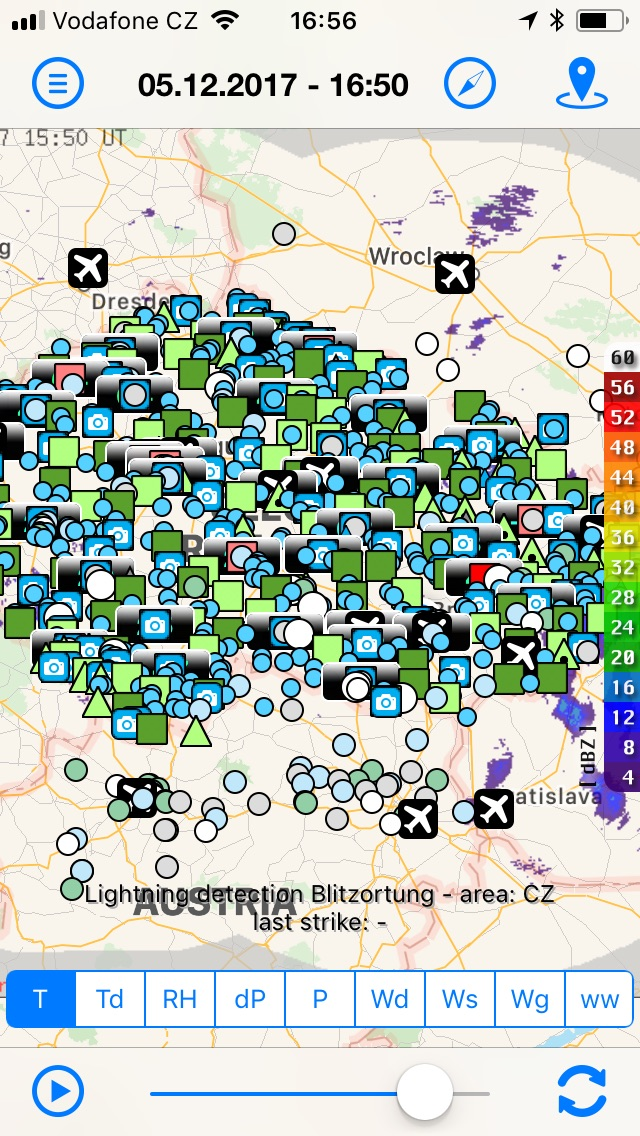
\includegraphics[width=0.75\textwidth]{all-layers}
        \caption{Map with all enabled layers.}
        \label{fig:all}
    \end{minipage}
    \hfill
    \begin{minipage}[b]{0.49\textwidth}
    \centering
        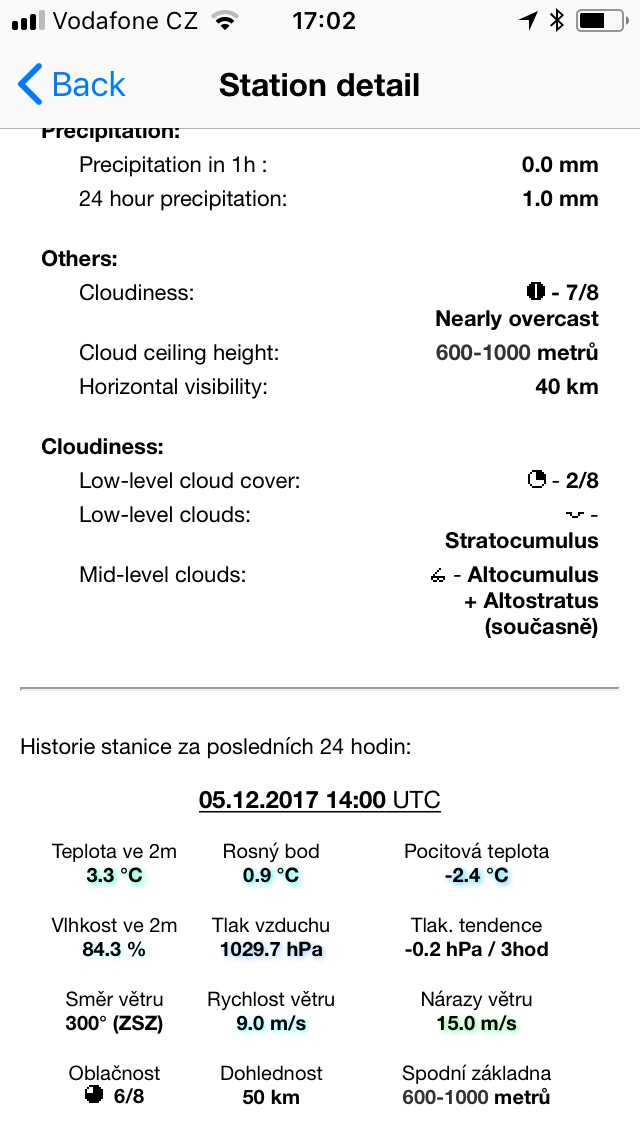
\includegraphics[width=0.75\textwidth]{czenglish}
        \caption{Mixture of Czech and English.}
        \label{fig:czeng}
    \end{minipage}


\end{figure}

\section{Summary}

To sum up the iRadar CZ+ application I would say it is one of the best apps for rainfall data on the App Store, even with its mistakes, for people living in the Czech Republic. I really admire the completely free of charge model even without displaying ads. Other weather app makers have several ads placed on the screen which really breaks the user experience when viewing full-size rainfall maps.

\bibliography{doc}{}
\bibliographystyle{abbrv}

\end{document}
